\section{Technical Section}

\subsection{Graph Model}

\begin{figure}[h]
	\centering
	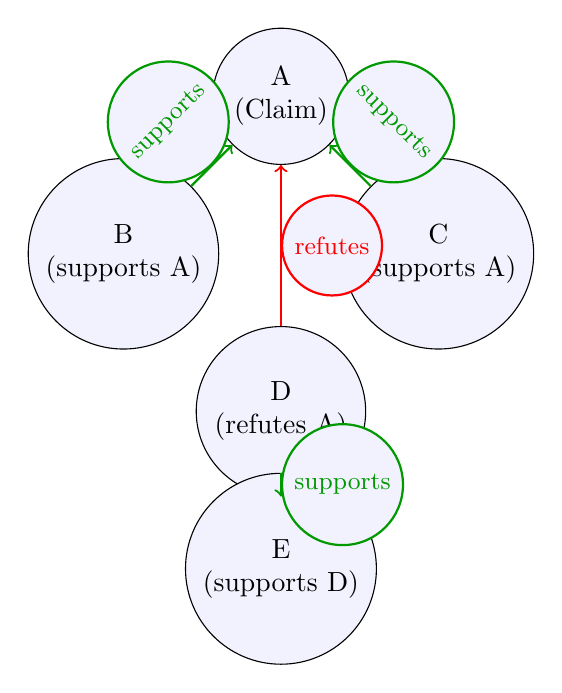
\begin{tikzpicture}[node distance=2.0cm and 2.5cm, every node/.style={draw, circle, fill=blue!5, minimum size=1cm, align=center}]
		\node (A) at (0,0) {A\\(Claim)};
		\node (B) at (-2,-2) {B\\(supports A)};
		\node (C) at (2,-2) {C\\(supports A)};
		\node (D) at (0,-4) {D\\(refutes A)};
		\node (E) at (0,-6) {E\\(supports D)};
		\draw[->, thick, green!60!black] (B) -- (A) node[midway, above, sloped]{\small supports};
		\draw[->, thick, green!60!black] (C) -- (A) node[midway, above, sloped]{\small supports};
		\draw[->, thick, red] (D) -- (A) node[midway, right]{\small refutes};
		\draw[->, thick, green!60!black] (E) -- (D) node[midway, right]{\small supports};
	\end{tikzpicture}
	\caption{Example evidence graph fragment. Node A represents an initial claim. Nodes B and C provide supporting evidence for A (green arrows). Node D provides a refuting evidence against A (red arrow). Node E supports the findings of D (i.e., replicates D's refutation of A). In the ASB system, this network of support and refutation relationships would be used to compute fragility scores for each node.}
	\label{fig:graph}
\end{figure}

In ASB, every research publication (or scientific claim) is represented as a node in a directed graph. We call this the \textbf{evidence graph}. An edge from node $B$ to node $A$ indicates that publication $B$ has cited publication $A$. However, unlike traditional citation indexes that do not distinguish the nature of the citation, ASB requires each citation to be annotated with its \emph{polarity}:
\begin{itemize}
	\item \textbf{Support}: If $B$'s findings \textit{support}, reproduce, or are consistent with the claims of $A$.
	\item \textbf{Refute}: If $B$'s findings \textit{contradict}, falsify, or cast serious doubt on the claims of $A$.
\end{itemize}
Each node can thus accumulate incoming links of either type over time as new papers cite it. These links form chains of evidence: for example, a paper $C$ might support paper $B$ which in turn refuted paper $A$, creating a sequence of evidence relationships.

Figure~\ref{fig:graph} illustrates a fragment of such an evidence graph. Each link is labeled as supporting (green arrow) or refuting (red arrow) evidence. This structure encodes not just which papers are connected, but the \emph{stance} of that connection, which is crucial for assessing credibility. A paper with many independent supporting replications will look very different in this graph from one that has attracted a well-substantiated refutation.

Importantly, this evidence graph is intended to be \textbf{open and evolving}. Anyone can add a new node (publish a new result) that cites prior work with appropriate support/refute designations. There is no central authority deciding which evidence is allowed; instead, the network grows organically as knowledge progresses. The graph provides a living documentation of the state of scientific testing for each claim. As evidence accumulates, the structure of the graph tells the story of how that claim has stood up (or faltered) under scrutiny.



\subsection{Evidence Fragility Score (EFS) algorithm}
The Evidence Fragility Score (EFS) is calculated by a trustless and recursive algorithm designed to evaluate the strength, transparency, and falsifiability of a research object without relying on consensus, reputation, or human authority.

EFS operationalizes the principle that textbf{falsifications are more epistemically significant than confirmations}. For example, if a claim $A$ has, say, five papers supporting it and no refutations, its ASB might be moderately high. But if a sixth paper comes along and refutes $A$ with strong evidence, that single refutation could outweigh the five supports, dramatically lowering $A$'s score. The refuting paper itself would receive a high score for providing compelling negative evidence. In effect, the system is constantly asking: "Has this claim been robustly challenged, and if so, did it withstand the test?" A claim that continues to be supported and never strongly refuted will see its score rise over time, whereas a claim that is refuted (or whose supporting evidence is undermined by later findings) will see its score fall.

Moreover, the \textbf{graph structure and the recursive nature of the EFS algorithm allows for the propagation of impact}. If a research $A$ is refuted by $D$, not only is $A$'s score reduced, but any other research $B$ that heavily relied on $A$ (say $B$ supported $A$ or built upon $A$'s result) may also suffer a hit to its EFS score, because one of the pillars supporting $B$ has cracked. EFS can capture this by dynamically recomputing scores so that the repercussions of new evidence ripple through the network. Over time, this helps prevent entire lines of research from resting on a faulty result: the moment the result is invalidated, the dependent work is flagged (via lowered scores) unless it can stand independently. 

\subsubsection{How It Works}
Each Research object carries metadata fields that describe its transparency, exposure to adversarial testing, funding conditions, and epistemic risk. 

The EFS algorithm combines the following key factors:
\begin{itemize}
	\item A local validation score - relates to Popper's falsifiability concept
	\item An antifragile funding score - relates to Taleb's \emph{skin in the game} concept and also the \emph{agent-principal problem}.
	\item An antifragile ruin score - to take into account the cost of being wrong.
	\item Recursive analysis of all linked research replications and refutations.
\end{itemize}

\subsubsection{Research Object Fields}
\begin{description}
	\item[\texttt{ruin\_scale}] Enum: \texttt{low}, \texttt{medium}, \texttt{high}. Used to calculate the ruin score dynamically.
	\item[\texttt{ruin\_impact}] Enum: \texttt{low}, \texttt{medium}, \texttt{high}. Used to calculate the ruin score dynamically.
	\item[\texttt{funders}] Array of objects. Each funder includes:
	\begin{itemize}
		\item \texttt{wallet\_id}: String. The identifier of the wallet.
		\item \texttt{anon}: Boolean. Whether the wallet is anonymous.
		\item \texttt{wallet\_age}: Integer. Wallet age in days.
		\item \texttt{amount}: Float. Amount funded.
	\end{itemize}
	\item[\texttt{data\_openness}] Enum: \texttt{none}, \texttt{partial}, \texttt{full}. Indicates the level of access to raw data and methods.
	\item[\texttt{validation\_enabled}] Boolean. Whether the research exposes raw data, methods, and test logic.
	\item[\texttt{test\_vectors}] Boolean. Whether test inputs and expected outputs are provided.
	\item[\texttt{refutations}] Count of formal, timestamped refutations logged on-chain.
	\item[\texttt{replications}] Count of successful replications with hash-verified results.
	\item[\texttt{research\_file\_url}] String. URL of the main research paper.
	\item[\texttt{research\_file\_hash}] String. Cryptographic hash of the research paper.
	\item[\texttt{data\_files}] Array of objects. Each object includes:
	\begin{itemize}
		\item \texttt{url}: String. URL where a dataset is stored.
		\item \texttt{hash}: String. Hash of the dataset to ensure integrity.
	\end{itemize}
\end{description}


\subsubsection{Validation Score}
\[
\text{validation}(R) = \mathbf{1}_{\text{validation\_enabled}} \cdot 0.4 + \text{data\_openness\_score} + \mathbf{1}_{\text{test\_vectors}} \cdot 0.2 + \log_2(n_{\text{rep}} + 1) \cdot 0.05 - n_{\text{ref}}
\cdot 0.1
\]

\subsubsection{Antifragile Funding Score}

Let $R$ contain a set of funders $F = \{f_1, f_2, \dots, f_n\}$, where each funder $f_i$ is a tuple $(\text{anon}_i, \text{wallet\_age}_i, \text{amount}_i)$. Then the funding score is computed as the
weighted average over all funders:

\[
\text{funding}(R) = \frac{\sum_{i=1}^{n} \text{amount}_i \cdot \left(1 - 0.2 \cdot \text{anon}_i - 0.1 \cdot \mathbf{1}_{\text{wallet\_age}_i < 30}\right)}{\sum_{i=1}^{n} \text{amount}_i}
\]

\subsubsection{Antifragile Ruin Score}
Let $\texttt{ruin\_scale}, \texttt{ruin\_impact} \in \{\texttt{low}, \texttt{medium}, \texttt{high}\}$. The final ruin score is computed as:

\[
\text{ruin}(R) = 1.0 + 0.25 \cdot \text{scale}(\texttt{ruin\_scale}) + 0.25 \cdot \text{impact}(\texttt{ruin\_impact})
\]

Where:
\begin{itemize}
	\item $\text{scale}(\texttt{low}) = 0$, $\texttt{medium} = 1$, $\texttt{high} = 2$
	\item $\text{impact}(\texttt{low}) = 0$, $\texttt{medium} = 1$, $\texttt{high} = 2$
\end{itemize}

This results in $\text{ruin}(R) \in [1.0, 2.0]$.

\subsubsection{The EFS Algorithm}
Let $R$ be a Research object. Then:
\[
\text{EFS}(R) =
\begin{cases}
	0 & \text{if } \text{isValid}(R) = \text{false} \\
	\frac{\text{validation}(R) \cdot \text{funding}(R)}{\text{ruin}(R)} + \sum_{i=1}^{m} \mathbf{1}_{\text{isValid}(R_i^{(\text{rep})})} \cdot \log_2(\text{EFS}(R_i^{(\text{rep})}) + 1) \cdot w_{\text{rep}}
	\\ - \sum_{j=1}^{n} \mathbf{1}_{\text{isValid}(R_j^{(\text{ref})})} \cdot \text{EFS}(R_j^{(\text{ref})}) \cdot w_{\text{ref}} & \text{otherwise}
\end{cases}
\]

Where:
\begin{itemize}
	\item $w_{\text{rep}}$: weight per replication (e.g., $0.05$)
	\item $w_{\text{ref}}$: weight per refutation (e.g., $0.1$)
\end{itemize}
